\section{RELATED WORK} \label{relatedwork}

Since their appearance in literature, GANs have been successfully applied to problems of image generation, editing and semi-supervised learning \cite{DBLP:journals/corr/RadfordMC15} \cite{DBLP:journals/corr/ZhangXLZHWM16}.
Results obtained were so promising that the new framework captured the interest of many researchers, leading to a proliferation of various flavors of GAN, each claiming to have better performances on a specific domain.
It's difficult anyway to understand how to compare different GAN models, because of the lack of a consistent metric and the different architectures networks can be designed with, which for each project are related to the corresponding computational budget.
A tentative to define some guidelines to avoid these problems, together with a fair and comprehensive comparison of state-of-the-art GANs, is discussed in \cite{46506}: what emerges here is that the computational budget plays a major role, allowing bad algorithms to outperform good ones if given enough time; plus, despite the many claims of superiority, there's no empirical evidence that those algorithms are better across all datasets, in fact in most of the cases the original model outperforms the others.
We thus report here a formalization of the original problem \cite{NIPS2014_5423}, modeling it with a game theory approach in a more precise way, as done in \cite{2017arXiv171200679O}.

GANs exploit as players (named G and D) the learning capability of neural networks. The two anyway have different purposes, so in general they are designed with different architectures (e.g. as in fig.\ref{fig:netG} and fig.\ref{fig:netD}).
As suggested in \cite{NIPS2014_5423}, the generator's distribution $p_g$ over data $x$ is learnt defining a prior on input noise variables $p_z(z)$ and representing the mapping to the data space as $G(z;\theta_g)$, where $\theta_g$ stands for the weights of the network.
Similarly for the discriminator, a mapping $D(x;\theta_d)$ can be defined from the data space to a scalar, also referred to as $D(x)$, representing the probability that the input belongs to the true distribution $p_{data}$, i.e. to the training set.
In the formalization of the game then, pure strategies are defined by the sets of possible $\theta_g$ and $\theta_d$, while the utilities functions are the opposite of the loss functions that the networks have to minimize.

For classification tasks, cross-entropy loss function is universally accepted as the best choice, giving good results in terms of learning speed: this is what is usually selected for D in GANs.
The simplest design of GAN uses as loss function for G the opposite of D's, defining thus a zero-sum game (MM-GAN).
Ideally, the number of strategies for each player would be infinite but, as pointed out in  \cite{2017arXiv171200679O}, when using floating point numbers it becomes finite, albeit very large: the game is then finite, implying the existence of a NE, at least in mixed strategies.
It has to be kept into account also the fact that the optimization of a neural network can lead to a Local NE (LNE) because the problem is non-convex.
We can then solve the equilibrium problem by computing the minimax of the payoffs.
Loss functions are defined as:
\begin{equation*}
	\begin{split}
		L^{(D)} = &-\mathbb{E}_{x \sim p_{data}(x)}[\log D(x)]\\
		          &- \mathbb{E}_{z \sim p_{z}(z)}[\log (1-D(G(z)))];\\
		L^{(G)} = &- L^{(D)},
	\end{split}
\end{equation*}
where, the expectations are computed on mini-batches of data.
For the very definition of cross-entropy loss function, $L^{(G)}$ can be simplified because all the samples are generated according to the same distribution: 
\begin{align*}
L^{(G)} = \mathbb{E}_{z \sim p_{z}(z)}[\log (1-D(G(z)))].
\end{align*}
The value of the game is defined as $V(G,D)=-L^{(D)}$.
Fixing a generator $\bar{G}$, the optimal discriminator can be computed maximizing D's utility, which corresponds to $V(\bar{G},D)$:
\begin{align*}
D^*(x) = \argmax\limits_{D} \big\{V(\bar{G},D) \big\}.
\end{align*}
Assuming that the model has infinite capacity in representing pdfs, we can study the convergence to a NE point in the space of pdf:
\begin{equation*}
\begin{split}
V(\bar{G},D) & = \int_x p_{data(x)} \log(D(x)) dx +\\
             & \ \ \ + \int_z p_{z}(z) \log(1-D(\bar{G}(z))) dz\\
             & = \int_x\Big[p_{data(x)} \log(D(x)) +\\
             & \ \ \ + p_{g}(x) \log(1-D(x)) \Big]dx\\
             & = \int_x L\big(x,D(x),\dot{D}(x)\big)dx.
\end{split}
\end{equation*}
$D^*(x)$ must satisfy the Euler-Lagrange equation:
\begin{align*}
	\frac{\partial L}{\partial D} = \frac{d L}{d x} \frac{\partial L}{\partial \dot{D}}
\end{align*}
and since $\partial L / \partial \dot{D} = 0$ we get:
\begin{align*}
	\frac{\partial L}{\partial D} = \frac{p_{data}(x)}{D(x)} - \frac{p_g(x)}{1-D(x)} = 0
\end{align*}
that implies:
\begin{align*}
	D^*(x) = \frac{p_{data}(x)}{p_{data}(x) + p_g(x)}.
\end{align*}
Minimizing then over $p_g(x)$, a point of minimum is found for $p_g = p_{data}$, where $V(G^*,D^*)=-\log(4)$ as proved in \cite{NIPS2014_5423}.

Cross-entropy loss functions are particularly effective for discrimination tasks, but they're not for generation ones because, in the beginning of the training phase, when G is poor and D is able to correctly recognize generated samples, $\log(1-D(G(z)))$ \textit{saturates} to zero, thus resulting in a poor gradient for backpropagation. The learning in that case is too slow, but this problem can be avoided changing the loss function for G: instead of minimizing $\log(1-D(G(z)))$, we can maximize $\log(D(G(z)))$. This is formally defined as a Non-Saturating GAN (NS-GAN), where the losses to be minimized are:
\begin{equation*}
\begin{split}
L^{(D)} = &-\mathbb{E}_{x \sim p_{data}(x)}[\log D(x)]\\
&- \mathbb{E}_{z \sim p_{z}(z)}[\log (1-D(G(z)))];\\
L^{(G)} = &- \log(D(G(z))),
\end{split}
\end{equation*}

This new game isn't zero-sum any more, but the same equilibrium point of the dynamics can be found as before, thus providing the same theoretical results.

\begin{figure}
	\begin{center}
		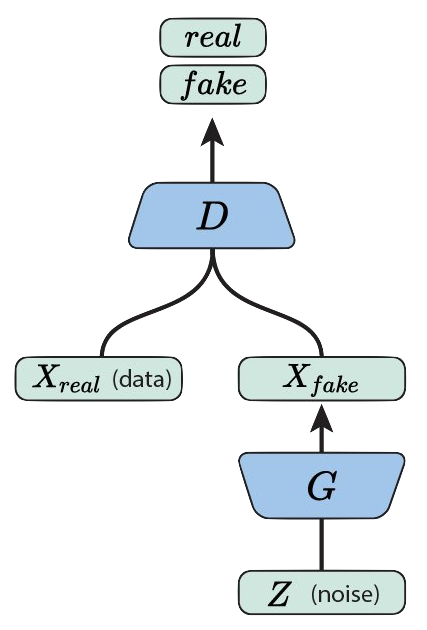
\includegraphics[scale=0.25]{./plots/GAN_model.png}
	\end{center}
	\caption{a block-diagram representing generative adversarial networks. A generator network ($G$) creates samples in data space from noise $z$. A discriminator network ($D$) then compares data, trying to distinguish true from fake samples.}
	\label{fig:game}
\end{figure}
\begin{figure}
	\begin{center}
		\includegraphics*[scale=0.35]{./plots/G_model.png}	
	\end{center}
	\caption{a high-level representation of G, the generator network, with 4 hidden layers. Each circle represents a perceptron unit in the network. A random vector of dimensionality 2, i.e. input noise, is transformed into a 28x28 grayscale image. The architecture presented is also used in our implementation of the model.}
	\label{fig:netG}
\end{figure}
\begin{figure}
	\begin{center}
		\includegraphics*[scale=0.35]{./plots/D_model.jpg}		
	\end{center}
	\caption{a high-level representation of D, the discriminator network, with 4 hidden layers. Each circle represents a perceptron unit in the network. 28x28 grayscale images are transformed into a scalar in range $[0,1]$, representing the probability of the image being true. The architecture presented is also used in our implementation of the model.}
	\label{fig:netD}
\end{figure}